% SIAM Article Template
\documentclass[r]{siamart171218}
% Packages and macros go here
\usepackage[english]{babel}
\usepackage{fullpage}
\usepackage{amsmath}
\usepackage{amssymb}
\usepackage{amsfonts}
\usepackage{array}
\usepackage{epsfig}
\usepackage{float}
\usepackage{fullpage}
\usepackage{color}
\usepackage{enumitem}  
\usepackage{epstopdf}
\usepackage{tikz}
\usepackage{multirow}
\usepackage{pgfplots}
\usepackage{standalone}
\usepackage{graphicx}
\usepackage{graphics}
\usepackage{color}

\usepackage{ifpdf}
\ifpdf
\DeclareGraphicsRule{*}{mps}{*}{}
\fi


\DeclareRobustCommand{\figlegend}[1]{%
  \raisebox{0.5ex}{
    \tikz[]{%
      \fill[very thick, color=#1] (0, 0) rectangle (0.3, 0.1);
    }%
  }
}
% Title. If the supplement option is on, then "Supplementary Material"
% is automatically inserted before the title.
%\title{On the weak coupling of 3D and 1D second order elliptic problems}
\title{Notes on robust solvers for systems of coupled multiscale PDEs}

% Authors: full names plus addresses.
\author{
Miroslav Kuchta, Federica Laurino, Kent-Andre Mardal, Paolo Zunino,\thanks{Authors are listed in alphabetical order}
}

\newcommand{\Miro}[1]{\textcolor{cyan}{Miro: #1}}

\begin{document}

\maketitle

% REQUIRED
\begin{abstract}
  We summarize numerical experiments related to the task of developing
  mesh and parameter indepent solvers for the 3$d$-1$d$ coupled diffusion problems.
  These are personal notes written to keep track of the developments on this
  topic and are to be kept confidential.
\end{abstract}

% REQUIRED
\begin{keywords}
elliptic problems, high dimensionality gap, essential coupling conditions, Lagrange multipliers
\end{keywords}

% REQUIRED
\begin{AMS}
n.a.
\end{AMS}

% >>>>>>>>>>>>>>>>>>>>>>>>>>>>>>>>>>>>>>>>>>>>>>>>>>>>>>>>>>>>>>>>>>>>>>>>>>>>>>>>>>>>>>>>>>>>>>>>>>>>

\newcommand{\MK}[1]{\textcolor{cyan}{#1}}

\newcommand{\semi}[1]{\lvert{#1}\rvert}
\newcommand{\norm}[1]{\lVert{#1}\rVert}
\newcommand{\jump}[1]{\ensuremath{[\![#1]\!]} }
\newcommand{\avg}[1]{\ensuremath{\left\{\!\left\{#1\right\}\!\right\}} }

\def\ud{u_{\odot}}
\def\vd{v_{\odot}}
\def\ld{\lambda_{\odot}}
\def\md{\mu_{\odot}}
\def\lld{l_{\odot}}
\def\uf{u_{\ominus}}
\def\up{u_{\oplus}}
\def\eps{\epsilon}
\def\nn{\boldsymbol n}
\def\rr{\boldsymbol r}
\def\RR{\boldsymbol R}
\def\kk{\boldsymbol k}
\def\ss{\boldsymbol s}
\def\uu{\boldsymbol u}
\def\vv{\boldsymbol v}
\def\xx{\boldsymbol x}
\def\bu{\overline{u}}
\def\bv{\overline{v}}
\def\tu{\widetilde{u}}
\def\tv{\widetilde{v}}
\def\TT{\boldsymbol T}
\def\NN{\boldsymbol N}
\def\BB{\boldsymbol B}
\def\ttu{\widetilde{\widetilde{u}}}
\def\ttv{\widetilde{\widetilde{v}}}
\def\cv{\check{v}}
\def\mesh{{\cal T}^h}
\def\ball{{\cal B}}
\def\R{\mathbb{R}}
\def\D{\mathcal{D}}
\def\DD{\partial\mathcal{D}}
\def\trace{{\mathcal{T}_\Gamma}}
\def\mtrace{{\overline{\mathcal{T}}_\Lambda}}
\def\ext{\mathcal{E}_\Gamma}
\def\ide{\mathcal{I}}
\def\ii{\hat{\imath}}
\newcommand{\avrd}[1]{\overline{\overline{#1}}}
\newcommand{\avrc}[1]{\overline{#1}}
\newcommand{\refe}[1]{{#1}_{\mathrm{ref}}}

\newcommand{\vertiii}[1]{{\left\vert\kern-0.25ex\left\vert\kern-0.25ex\left\vert #1 
    \right\vert\kern-0.25ex\right\vert\kern-0.25ex\right\vert}}


\newtheorem{thm}{Theorem}[section]
\newtheorem{prop}{Property}[section]
\theoremstyle{remark}
\newtheorem{remark}{Remark}[section]

\newtheorem{example}{Example}[section]

\section{Introduction}\label{sec:intro}

Let $\langle \cdot , \cdot \rangle_\Lambda$ denote the duality pairing between 
$H^\frac12_{00}(\Lambda)$ and $H^{-\frac12}(\Lambda)$. This note concerns robust
solvers for the problem:
Find $u \in H^1_0(\Omega),\ \ud \in H^1_0(\Lambda), \ \ld \in H^{-\frac12}(\Lambda)$, such that
\begin{subequations}\label{eq:problem2}
\begin{align}
&(u,v)_{H^1(\Omega)} + (\ud,\vd)_{H^1(\Lambda),|\D|} 
+  \langle \mtrace v - \vd, \ld \rangle_{H^{-\frac12}(\Lambda), |\DD|} 
\\
\nonumber
&\qquad\qquad= (f,v)_{L^2(\Omega)} +  (\avrd{g},V)_{L^2(\Lambda),|\D|}
\quad \forall v \in H^1_0(\Omega), \ \vd \in H^1_0(\Lambda)\,,
\\
&   \langle \mtrace u -   \ud, \md \rangle_{H^{-\frac12}(\Lambda),|\DD|} = 0
\quad \forall \md \in H^{-\frac12}(\Lambda)\,,
\end{align}
\end{subequations}
where $\mtrace$ denotes the composition of operators $\avrc{(\cdot)} \circ \trace $.
In particular, we aim at devising algorithms that are robust with respect to
the averaging radius in $\mtrace$.

The (continuous) problem \eqref{eq:problem2} is well posed, in particular
the Lagrange multiplier $\md$ exists in a suitable fractional Sobolev space on
$\Lambda$. Following operator preconditioning framework \cite{mardal2011preconditioning} preconditioners
for the problem rely on fractional Sobolev norms. At the moment the stability
of the discrete problem can be shown using the Lagrange multiplier defined
in the space of piecewise constant functions over the collection of tetrahedra
(of the 3$d$ mesh) that are intersected by $\Lambda$. However, it is not clear
how fractional Sobolev norms on such a space should be constructed (in contrast
to the case where the multiplier is defined on $\Lambda$). We shall therefore
establish the preconditioners for the \emph{discrete} problem using different
norms than those used in the analysis of the \emph{continuous} one.

As a stepping stone to \eqref{eq:problem2} we shall consider a related
2$d$-1$d$ problem\\
%Stong
\begin{minipage}{0.57\textwidth}
  \begin{equation}\label{eq:coupled}
    \begin{aligned}
      -\Delta u^i &= f &\mbox{ in }\Omega^{i}, i\in\left\{+, -\right\},\\
      \jump{u} &= 0 &\mbox{ on }\Gamma,\\
      -\Delta \hat{u} +\hat{u} - \jump{\nabla u\cdot n}&= \hat{f} &\mbox{ on }\Gamma,\\
      \epsilon u - \hat{u} &= h&\mbox{ on }\Gamma.\\
    \end{aligned}
\end{equation}
\null
\par\xdef\tpd{\the\prevdepth}
\end{minipage}
\hfill
\begin{minipage}{0.37\textwidth}
  \begin{figure}[H]
    \begin{center}
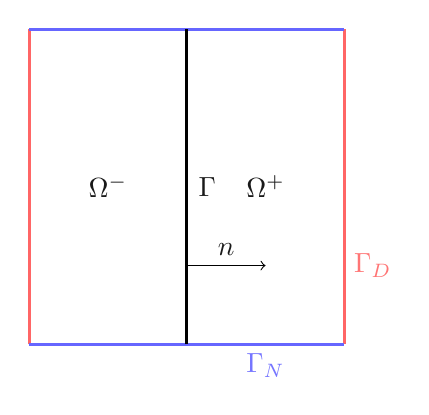
\begin{tikzpicture}
  \node[black, fill=white, opacity=0.9] at (1, 2) {$\Omega^{-}$};
  \node[black, fill=white, opacity=0.9] at (3, 2) {$\Omega^{+}$};

  % Boundaries
  \draw[very thick, red!60!white] (0, 0) -- (0, 4);
  \draw[very thick,red!60!white] (4, 0) -- (4, 4);
  \node[red!60!white, opacity=0.9, right] at (4, 1) {$\Gamma_D$};

  \draw[very thick, blue!60!white] (0, 0) -- (4, 0);
  \draw[very thick, blue!60!white] (0, 4) -- (4, 4);
  \node[blue!60!white, opacity=0.9, below] at (3, 0) {$\Gamma_N$};

  \draw[black, very thick] (2, 0) -- (2, 4);
  \draw[->, black] (2, 1) -- (3, 1);
  \node[fill=white, opacity=0.9, above] at (2.5, 1) {$n$};
  \node[fill=white, opacity=0.9, right] at (2.025, 2) {$\Gamma$};
\end{tikzpicture}
    \end{center}
    %\vspace{-20pt}
    \caption{Schematic domain of coupled multiscale problem.}
    \label{fig:coupled_domain}
    %\vspace{5pt}    
\end{figure}
\end{minipage}
%
Here \eqref{eq:coupled} shall be equipped with Dirichlet boundary conditions
(for $u^i$) on $\Gamma_D$, while Neumann conditions are used on $\Gamma_N$
(for both the unknowns). Note that the role of constant parameter $\epsilon$ is similar
to that of averaging radius in \eqref{eq:problem2}.

Let $\Omega=\Omega^{+}\cup\Omega^{-}$. Introducing a Lagrange multiplier
$p=\epsilon^{-1}\jump{\nabla u \cdot n}\in Q=H^{-1/2}(\Gamma)$
the weak form of \eqref{eq:coupled} reads: Find $u\in V=H^1_{0, \Gamma_D}(\Omega)$,
$\hat{v}\in\hat{V}=H^1(\Gamma)$, $p\in Q$ such that
%
\begin{equation}\label{eq:coupled_weak}
  \begin{aligned}
    &\int_{\Omega}\nabla u\cdot \nabla v\,\mathrm{d}x &\phantom{+\int_{\Gamma}\nabla \hat{u}\cdot \nabla \hat{v}} &+\epsilon\int_{\Gamma} p v\,\mathrm{d}s &= \int_{\Omega}f v\,\mathrm{d}x \quad &\forall v\in V,\\
    &\phantom{\int_{\Omega}\nabla u\cdot \nabla v} &+{\int_{\Gamma}\nabla \hat{u}\cdot \nabla \hat{v} + \hat{u}\hat{v}\,\mathrm{d}s} &-\int_{\Gamma} p\hat{v}\,\mathrm{d}s &= \int_{\Gamma}\hat{f}\hat{v}\,\mathrm{d}s \quad &\forall \hat{v}\in \hat{V},\\
    &\epsilon\int_{\Gamma}u q\,\mathrm{d}s &-\int_{\Gamma}\hat{u}q\,\mathrm{d}s &\phantom{-\int{\Gamma}q\hat{v}} &= \int_{\Gamma}h q\,\mathrm{d}s \quad &\forall q\in Q.
  \end{aligned}
\end{equation}

In the following it will be convenient to work with the operator form of
\eqref{eq:coupled_weak}. In particular the left-hand-side defines an operator
%
\begin{equation}\label{eq:operator2d}
  \mathcal{A} = \begin{pmatrix}
    -\Delta_{\Omega} & & \epsilon T^{\prime}\\
    & -\Delta_{\Gamma} + I & -I\\
    \epsilon T & -I & \\
  \end{pmatrix} =
  \begin{pmatrix}
    A_2 &  & B_2'\\
    & A_1 & -B_1'\\
    B_2 & -B_1 & \\
   \end{pmatrix}.
\end{equation}
In \cite{kuchta2016preconditioners} it is shown that $\mathcal{A}$ is an
isomorphism from $W$ to its dual space where
\[
W=H^1(\Omega)_{0, \Gamma_D}\times H^1{(\Gamma)}\times(\epsilon H^{-1/2}(\Gamma)\cap H^{-1}(\Gamma)).
\]
It is further shown that discretization in terms of continuous linear Lagrange
elements (P1) for all the unknowns is inf-sup stable and in turn the diagonal operator
\begin{equation}\label{eq:P1_precond}
\mathcal{B}=\text{diag}(-\Delta_{\Omega}, -\Delta_{\Gamma}+I, \epsilon^2(-\Delta_{\Gamma})^{-1/2}+(-\Delta_{\Gamma}+I)^{-1})^{-1}
\end{equation}
is a robust preconditioner for $\mathcal{A}$. For the sake of completness
(and verifying the implementation) Table \ref{tab:P1} shows the number of
MinRes iterations and condition numbers\footnote{
  Unless specified otherwise all the experiments are done on $\Omega$ a unit square
  triangulated into $2N^2$ isosceles triangles. MinRes iterations are always started
  from a random initial vector and terminate once the relative preconditioned residual
  norm is reduced by factor $10^{8}$. Condition numbers of the preconditioned problem
  are computed by direct solver, i.e. from the full spectrum.
} of the preconditioned problem for
different levels of refinement and values of the parameter $\epsilon$. The
stability is evident.
%
\begin{table}
    \footnotesize{
      \begin{minipage}{0.49\textwidth}
          \begin{center}
            \begin{tabular}{c|cccc} \hline
              \multirow{2}{*}{$\epsilon$} & \multicolumn{4}{c}{$h$}\\
              \cline{2-5}
 &   $2^{-2}$  & $2^{-3}$ & $2^{-4}$ & $2^{-5}$   \\  
\hline
$10^{6}$ &	7.73&	7.82&	7.86&	7.87\\
$10^{4}$ &	7.73&	7.82&	7.86&	7.87\\
$10^{2}$   &	7.73&	7.82&	7.86&	7.87\\
1     &	7.39&	7.79&	8.01&	8.13\\
$10^{-2}$  &	2.62&	2.63&	2.63&	2.65\\
$10^{-4}$ &	2.62&	2.62&	2.62&	2.62\\
$10^{-6}$ &	2.62&	2.62&	2.62&	2.62\\
\hline
\end{tabular}
\end{center}
      \end{minipage}
    }
          \footnotesize{
            \begin{minipage}{0.49\textwidth}
              \begin{center}
            \begin{tabular}{c|cccccc} \hline
              \multirow{2}{*}{$\epsilon$} & \multicolumn{6}{c}{$h$}\\
              \cline{2-7}
 &   $2^{-3}$ & $2^{-4}$ & $2^{-5}$ & $2^{-6}$ & $2^{-7}$ & $2^{-8}$  \\  
              \hline
$10^{6}$ & 21 & 22 & 22 & 21 & 21 & 19\\
$10^{4}$ & 21 & 22 & 22 & 21 & 21 & 19\\
$10^{2}$ & 21 & 22 & 22 & 21 & 21 & 19\\
1 & 24 & 28 & 26 & 26 & 27 & 25\\
$10^{-2}$ & 10 & 10 & 10 & 12 & 13 & 14\\
$10^{-4}$ & 6 & 6 & 6 & 6 & 7 & 7\\
$10^{-6}$ & 4 & 4 & 4 & 4 & 4 & 4\\
\hline
\end{tabular}                
              \end{center}
        \end{minipage}
      }
          \caption{
            Problem \eqref{eq:coupled_weak} discretized with P1 elements.
            Condition number (left) and iterations counts (right) using
            preconditioner \eqref{eq:P1_precond}.
          }
          \label{tab:P1} 
%\label{table1}
\end{table}

Preconditioner \eqref{eq:P1_precond} was derived under the assumption that
the finite element mesh $\Gamma_h$ of $\Gamma$ consists of facets of the finite
element mesh $\Omega_h$ of $\Omega$, see also Figure \ref{fig:domains} (i). This
assumption is too limiting; for practical purposes the meshes should be independent
and a more common case is that the trace mesh of $\Omega_h$ on $\Gamma$ is coarser
than $\Gamma_h$. In the following we shall pursue formulations (and corresponding
solvers) of \eqref{eq:coupled_weak} which allow for different meshes and resolutions.
Our ultimate goal is a stable formulation in which the multiplier is not defined
on $\Gamma_h$ but rather on cells of $\Omega_h$ intersected by the curve, cf. Figure
\ref{fig:domains} (iv) and (v).
%
\begin{figure}
  \begin{center}
    \includegraphics[width=0.4\textwidth]{./img/conform.tex}\\

  \includegraphics[width=0.4\textwidth]{./img/conform_fine.tex}\hfill
  \includegraphics[width=0.4\textwidth]{./img/cut_fine.tex}\\
  \includegraphics[width=0.4\textwidth]{./img/nocut_lm2d.tex}\hfill
    \includegraphics[width=0.4\textwidth]{./img/cut_lm2d.tex}
  \end{center}
  \caption{Schematic geometric setting and discretization of multiscale problems.
    Position of interface $\Gamma$ is denoted by \figlegend{green!50!black}. Meshes
    underlying discrete approximation spaces $\hat{V}_h$ and $Q_h$ of $\hat{V}$ and $Q$ are denoted respectively
    by \figlegend{white!50!blue} and \figlegend{white!50!red}. Geometric correspondence
    is signified by dashed line. Cases: (i) trace mesh of $V_h$ is used for $\hat{V}_h$ and $Q_h$,
    (ii) $\Gamma$ does not intersect $\Omega_h $ cell interiors, (iii) $\Gamma$ does
    intersect cell interiors, (iv) as (ii) with $Q_h$ defined on intersected cells and
    (v) as (iii) with $Q_h$ defined on intersected cells.
  }
 \label{fig:domains}
\end{figure}

The rest of the report is structured as follows. Considering \eqref{eq:operator2d}
we first treat the problems related to domains $\Omega$, i.e. $\mathcal{A}_2=\left[A_2, B_2'; B_2, 0\right]$,
and $\Gamma$, i.e. $\mathcal{A}_1=\left[A_1, B_1'; B_1, 0\right]$, individually\footnote{This is done for
clarity of exposition, to better fix the ideas and debugging.}. More precisely, in
\S\ref{sec:problem_omega} a set of preconditioners for different formulations of the Babu{\v s}ka
problem is presented culminating in a formulation having the discrete Lagrange multiplier on the
cut cells. In \S\ref{sec:problem_gamma} we deal with instabities in $\mathcal{A}_1$ which arise
due to choices of discretization of the Lagrange multiplier space in $\mathcal{A}_2$. Finally in
\S\ref{sec:coupled} the insights from individual problems are combined to yield robust solvers
for the coupled problem.

\section{Preconditioning $\mathcal{A}_2$}\label{sec:problem_omega}
With Figure \ref{fig:coupled_domain} in mind we wish to solve the 2$d$-1$d$
coupled problem: Find $u\in V=H^1_{0, \Gamma_{D}}(\Omega)$,
$p\in Q=H^{-1/2}(\Gamma)$ such that
 %
\begin{equation}\label{eq:A2}
\begin{aligned}
  &\int_{\Omega}\nabla u\cdot\nabla v\,\mathrm{d}x + &{\int_{\Gamma}p v} &= \int_{\Omega}f v\,\mathrm{d}x\quad\forall v\in V,\\
  &{\int_{\Gamma}q u\,\mathrm{d}s} + &\phantom{\int{\Gamma}p v} &= \int_{\Gamma}g q\,\mathrm{d}s\quad\forall q\in Q.\\
\end{aligned},
\quad\mbox{or equivalently}\quad
\mathcal{A}_2\begin{pmatrix}
u\\
p\\
\end{pmatrix} = L.
\end{equation}
%
It can be seen that $\mathcal{A}_2$ is an isomorphism from $W=V\times Q$
to $W^{'}$ and in turn by \cite{mardal2011preconditioning} operator
\[
\mathcal{B}_2=\text{diag}(-\Delta_{\Omega}, (-\Delta_{\Gamma}+I)^{-1/2})^{-1}
\]
is a cannonical preconditioner for $\mathcal{A}_2$. Considering first the
case (i) from Figure \ref{fig:domains}, i.e. trace mesh of $\Omega_h$ is
$\Gamma_h$ and using (stable) P1-P1 discretization Table \ref{tab:A2} shows
that both the condition number and the number of MinRes iterations of $\mathcal{B}_2\mathcal{A}_2$
are bounded.

In order to arrive at the formulation where the discrete multiplier space
$Q_h$ is setup on the $\Gamma$-intersected cells of $\Omega_h$ let us first
consider an intermediate formulation with a piecewise constant (P0) multiplier defined
on $\Gamma_h$, cf. Figure \ref{fig:domains} (ii) and (iii). It is well known, e.g.
\cite[Ch 11.3]{steinbach2007numerical}, that if trace mesh of $\Omega_h$ is $\Gamma_h$ then P1-P0 discretization is
unstable. However the pair is stable if $\Gamma_h$ is coarser than the trace
mesh or a stabilization is employed. In the application we have in mind
the mesh of $\Omega$ is in general coarser than that of $\Gamma$ and thus
stabilized formulation is of interest. To highlight the difference in resolution
between the meshes we shall use different subscripts, i.e. $\Omega_H$ and
$\Gamma_h$. We remark that stabilization for piecewise linear Lagrange multipliers
(on $\Gamma$) is discussed in \cite{burman2009interior}.

Let $V_H=V_H(\Omega_H)$, $Q_h=Q_h(\Gamma_h)$ be the finite element approximations
of $V$ and $Q$ in terms of P1 and P0 elements respectively. Following \cite{burman2014projection}
the stabilized formulation of \eqref{eq:A2} reads: Find $u \in V_H$ and
$p \in Q_h$ such that
%
\[
\begin{aligned}
  &\int_{\Omega}\nabla u\cdot\nabla v\,\mathrm{d}x + &{\int_{\Gamma}p v\,\mathrm{d}s} &= \int_{\Omega}f v\,\mathrm{d}x\quad\forall v\in V_H,\\
  &{\int_{\Gamma}q u\,\mathrm{d}s} + &-\sum_{F\in\mathcal{F}}\int_{F}h^2\jump{p}\jump{q} \mathrm{d}s &= \int_{\Gamma}g q\,\mathrm{d}s\quad\forall q\in Q_h,\\
\end{aligned},
\quad\mbox{or equivalently}\quad
\mathcal{A}_{2, \Gamma_h}\begin{pmatrix}u\\p\\\end{pmatrix} = L.
\]
%
Here $\mathcal{F}$ is the union of internal and $\Gamma_N$-intersecting
facets of $\Gamma_h$. A possible preconditioner for $\mathcal{A}_{2,\Gamma_h}$,
which is based on the mapping properties of the continuous problem is a Riesz
map with respect to the inner product in induced by $\mathcal{B}^{-1}_{2, \Gamma_h}$
\[
\langle
\mathcal{B}^{-1}_{2, \Gamma_h}\begin{pmatrix}u\\p\end{pmatrix},
  \begin{pmatrix}v\\q\end{pmatrix}
\rangle
    =
    \int_{\Omega}\nabla u\cdot\nabla v\,\mathrm{d}x + \langle(-\Delta_{\Gamma}+I)^{-1/2}p, q\rangle
    + \sum_{F\in\mathcal{F}}\int_{F}h^2\jump{p}\jump{q} \mathrm{d}s.
\]
Robustness of the preconditioner can be seen in Table \ref{tab:A2} in both
the case where $\Gamma_h$ does not and does intersect the cell interior of $\Omega_h$ (cases
(iii) and (iv) in Figure \ref{fig:domains}). A potential difficulty with
$\mathcal{B}_{2, \Gamma_h}$ is, however, its generalization to the case of $Q_h$ defined
on intersected cells (interiors). In particular, the fractional norm can be
problematic. To avoid the issue, we therefore consider an alternative
preconditioner based on \cite[\S 4.A]{burman2014projection}
\[
\langle
\tilde{\mathcal{B}}^{-1}_{2, \Gamma_h}\begin{pmatrix}u\\p\end{pmatrix},
  \begin{pmatrix}v\\q\end{pmatrix}
\rangle
    =
    \int_{\Omega}\nabla u\cdot\nabla v\,\mathrm{d}x + \int_{\Gamma}h^{-1}u v\,\mathrm{d}s + \int_{\Gamma} h p q\,\mathrm{d}s
    + \sum_{F\in\mathcal{F}}\int_{F}h^2\jump{p}\jump{q} \mathrm{d}s.
\]
Note that the fractional norm on the multiplier has been replaced by the $h$-weighted
$L^2$ norm. Furthermore, there is an additional control of the trace of $u$ on
the curve by $h^{-1}$-weighted $L^2$ norm. We remark that \cite{burman2014projection} proves
the inf-sup condition for $\mathcal{A}_{2, \Gamma_h}$ using the norms on $V_H$ and
$Q_h$ as follows
\[
\norm{u}^2_{V_H} = \norm{\nabla u}^2_0 + \int_{\Gamma}h^{-1} u v\,\mathrm{d}s
\quad\mbox{and}\quad
\norm{p}_{Q_h} = \norm{h^{1/2} p}_0.
\]

Robustness of the preconditioner is
shown in Table \ref{tab:A2}; in the cut case (iii) the preconditioner is more
efficient than $\mathcal{B}_{2, \Gamma_h}$. We remark that the error convergence
of $\norm{u-u_H}_1$ is reduced in this case due to the fact that the kink
of the solution cannot be captured within the element.

Finally, we extend $\mathcal{A}_{2, \Gamma_h}$ to the formulation with Lagrange
mutliplier on the intersected elements. To this end, let $\mathcal{S}_H$ denote
elements of $\Omega_H$ intersected by $\Gamma_h$. The space $Q_H$ now consists
of piecewise constants on $\mathcal{S}_H$. Following \cite[\S 4.B]{burman2014projection}
we consider problem: Find $u\in V_H$, $p\in  Q_H$ such that
%
\[
\begin{aligned}
  &\int_{\Omega}\nabla u\cdot\nabla v\,\mathrm{d}x + &{\int_{\Gamma}p v\,\mathrm{d}s} &= \int_{\Omega}f v\,\mathrm{d}x\quad\forall v\in V_H,\\
  &{\int_{\Gamma}q u\,\mathrm{d}s} + &-\sum_{F\in\partial\mathcal{S}}\int_{F}H\jump{p}\jump{q} \mathrm{d}s &= \int_{\Gamma}g q\,\mathrm{d}s\quad\forall q\in Q_H,\\
\end{aligned},
\quad\mbox{or equivalently}\quad
\mathcal{A}_{2, \Omega_H}\begin{pmatrix}u\\p\\\end{pmatrix} = L.
\]
%
Here $\partial\mathcal{S}$ denotes interior and Neumann boundary intersecting
facets of $\mathcal{S}$. We remark that the norms for the inf-sup condition (shown
in \cite{burman2014projection} of $\mathcal{A}_{2, \Omega_H}$) are identical to $\mathcal{A}_{2, \Gamma_g}$.

Note that the stabilization is newly applied on edges
(points previously in $\mathcal{A}_{2, \Gamma_h}$) and relative to $\mathcal{A}_{2, \Gamma_h}$
we componsate for the increased dimensionality of the facets by decreasing
the exponent of the $H$-weight. In a similar manner
the preconditioner $\tilde{\mathcal{B}}_{2, \Gamma_h}$ can be generalized
yielding $\tilde{\mathcal{B}}_{2, \Omega_H}$
\[
\langle
\tilde{\mathcal{B}}^{-1}_{2, \Omega_H}\begin{pmatrix}u\\p\end{pmatrix},
  \begin{pmatrix}v\\q\end{pmatrix}
\rangle
    =
    \int_{\Omega}\nabla u\cdot\nabla v\,\mathrm{d}x + \int_{\Gamma}h^{-1}u v\,\mathrm{d}s + \int_{\Gamma} h p q\,\mathrm{d}s
    + \sum_{F\in\partial\mathcal{S}}\int_{F}H\jump{p}\jump{q} \mathrm{d}s.
\]
In Table \ref{tab:A2} we observe that MinRes iterations with
$\tilde{\mathcal{B}}_{2, \Omega_H}\mathcal{A}_{2, \Omega_H}$ are bounded. The decreasing
increments of the condition numbers suggest that $\kappa$ is bounded as well.

\begin{table}
    \scriptsize{% (i)
  \begin{center}
    \begin{tabular}{c|cccc}%||cc}
      \hline
      \multirow{2}{*}{$\frac{H}{H_0}$} & \multicolumn{4}{c}{$\mathcal{B}_2$}\\ %& \multicolumn{2}{c}{$\mathcal{B}_{h}$}\\
      \cline{2-5}
      & $\norm{u-u_H}_1$ & $\norm{\lambda-\lambda_H}_0$ & \#\\% & $\kappa$ & \# & $\kappa$\\
      \hline
1        & 8.62E-1(--)  & 1.04E0(--)    &   21 & 7.8\\ % & 24 & 20.9 \\
$2^{-1}$ & 4.4E-1(0.99) & 3.8E-1(1.46)  & 24   & 7.9\\ % & 41 & 21.1 \\
$2^{-2}$ & 2.2E-1(1.00) & 1.4E-1(1.49)  & 22   & 7.9\\ % & 46 & 21.2 \\
$2^{-3}$ & 1.1E-1(1.00) & 4.8E-2(1.50)  & 22   & -- \\ % & 47 & --   \\
$2^{-4}$ & 5.5E-2(1.00) & 1.7E-2(1.50)  & 21   & -- \\ % & 48 & --   \\
$2^{-5}$ & 2.7E-2(1.00) & 6.0E-3(1.50)  & 21   & -- \\ % & 45 & --   \\
\hline
  \end{tabular}
  \end{center}
    }
    \vspace{5pt}
  \scriptsize{%(ii)
    \begin{minipage}{0.49\textwidth}
  \begin{center}
    \begin{tabular}{c|cccc||cc}
      \hline
      \multirow{2}{*}{$\frac{H}{H_0}$} & \multicolumn{4}{c||}{$\mathcal{B}_{2, \Gamma_h}$} & \multicolumn{2}{c}{$\tilde{\mathcal{B}}_{2, \Gamma_h}$}\\
      \cline{2-7}
      & $\norm{u-u_H}_1$ & $\norm{\lambda-\lambda_h}_0$ & \# & $\kappa$ & \# & $\kappa$\\
      \hline
1       & 8.6E-1(--) & 5.4E-1(--)    & 29 & 6.5 & 25 & 16.9\\
$2^{-1}$ & 4.3E-1(0.98) & 2.3E-1(1.20)& 29 & 6.6 & 31 & 17.7\\
$2^{-2}$ & 2.2E-1(1.00) & 1.0E-1(1.19)& 28 & 6.6 & 34 & 18.1\\
$2^{-3}$ & 1.1E-1(1.00) & 4.7E-2(1.13)& 28 & --   & 37 & --   \\
$2^{-4}$ & 5.5E-2(1.00) & 2.2E-2(1.08)& 28 & --   & 37 & --   \\
$2^{-5}$ & 2.7E-2(1.00) & 1.1E-2(1.04)& 27 & --   & 37 & --   \\
\hline
  \end{tabular}
  \end{center}
  \end{minipage}
  }
    \scriptsize{%(iii)
    \begin{minipage}{0.49\textwidth}
  \begin{center}
    \begin{tabular}{c|cccc||cc}
      \hline
      \multirow{2}{*}{$\frac{H}{H_0}$} & \multicolumn{4}{c||}{$\mathcal{B}_{2, \Gamma_h}$} & \multicolumn{2}{c}{$\tilde{\mathcal{B}}_{2, \Gamma_h}$}\\
      \cline{2-7}
      & $\norm{u-u_H}_1$ & $\norm{\lambda-\lambda_h}_0$ & \# & $\kappa$ & \# & $\kappa$\\
      \hline
1       & 1.3E0(--)   & 1.7E0(--)    & 31 & 6.7 & 21 & 2.5\\
$2^{-1}$ &8.2E-1(0.68) & 9.2E-1(0.92)  & 32 & 6.6 & 21 & 2.5\\
$2^{-2}$ &5.4E-1(0.63) & 4.6E-1(1.00)  & 31 & 6.6 & 21 & 2.5\\
$2^{-3}$ &3.6E-1(0.58) & 2.3E-1(1.01)  & 30 & --  & 20 & --  \\
$2^{-4}$ &2.5E-1(0.54) & 1.1E-1(1.01)  & 28 & --  & 20 & --  \\
$2^{-5}$ &1.7E-1(0.52) & 5.7E-2(1.01)  & 28 & --  & 18 & --  \\
      \hline
  \end{tabular}
  \end{center}
  \end{minipage}
    }
    \vspace{5pt}
    \\
  \scriptsize{%(iv)
    \begin{minipage}{0.49\textwidth}
  \begin{center}
    \begin{tabular}{c|cccc}
      \hline
      \multirow{2}{*}{$\frac{H}{H_0}$} & \multicolumn{4}{c}{$\mathcal{B}_{2, \Omega_H}$}\\
      \cline{2-5}
      & $\norm{u-u_h}_1$ & $\norm{\lambda-\lambda_h}_0$ & \# & $\kappa$\\
      \hline
1       & 1.7E0(--)    & 2.0E0(--)    & 22 &4.5\\
$2^{-1}$ & 1.0E0(0.71)  & 1.2E0(0.71)  & 27 &5.1\\
$2^{-2}$ & 5.9E-1(0.78) & 7.7E-1(0.69) & 29 &5.4\\
$2^{-3}$ & 3.3E-1(0.85) & 4.9E-1(0.64) & 29 &-- \\
$2^{-4}$ & 1.7E-1(0.91) & 3.3E-1(0.59) & 28 &-- \\
$2^{-5}$ & 9.1E-2(0.95) & 2.2E-1(0.55) & 26 &-- \\
      \hline
  \end{tabular}
  \end{center}
  \end{minipage}
  }
  \scriptsize{%(iv)
    \begin{minipage}{0.49\textwidth}
  \begin{center}
    \begin{tabular}{c|cccc}
      \hline
      \multirow{2}{*}{$\frac{H}{H_0}$} & \multicolumn{4}{c}{$\mathcal{B}_{2, \Omega_H}$}\\
      \cline{2-5}
      & $\norm{u-u_h}_1$ & $\norm{\lambda-\lambda_h}_0$ & \# & $\kappa$\\
      \hline
1       & 2.0E0(--) & 1.3E0(--)        & 24 & 5.8\\
$2^{-1}$ & 1.4E0(0.53) & 7.0E-1(0.93)   & 29 & 7.1\\
$2^{-2}$ & 9.1E-1(0.62) & 3.5E-1(1.02)  & 34 & 8.0\\
$2^{-3}$ & 5.7E-1(0.68) & 1.6E-1(1.08)  & 36 & -- \\
$2^{-4}$ & 3.5E-1(0.71) & 7.9E-2(1.05)  & 36 & -- \\
$2^{-5}$ & 2.2E-1(0.69) & 4.3E-2(0.89)  & 34 & -- \\
      \hline
  \end{tabular}
  \end{center}
  \end{minipage}
  }
%%%%%%%%%%%%%
  \caption{Iteration counts (\#) and condition numbers ($\kappa$) of different
    preconditioned formulations of \eqref{eq:A2}, $H_0=2^{-4}$ and $h=H/3$.
    The cases correspond to setups (i)-(v) from Figure \ref{fig:domains}.
    First row (i) with $\mathcal{A}_2$. Second row (ii) and (iii) with
    $\mathcal{A}_{2, \Gamma_h}$. Third row (iv) and (v) with $\mathcal{A}_{2, \Omega_H}$.
  }
  \label{tab:A2}
\end{table}

At this point we have at our disposal an efficient solver for $\mathcal{A}_2$,
that is a 2$d$-1$d$ subcomponent of the coupled problem \eqref{eq:coupled_weak}.
We now turn attention to the 1$d$-1$d$ component; the idea being that the solver
for the coupled problem in some sense consists of solvers for $\mathcal{A}_2$ and
$\mathcal{A}_1$.


\section{Preconditioning $\mathcal{A}_1$}\label{sec:problem_gamma}
1


\section{Preconditioning 2$d$ coupled problem}\label{sec:coupled2d}
3


\section{Preconditioning 3$d$ coupled problem}\label{sec:coupled2d}
\input{coupled3d}


\bibliographystyle{siamplain}
\bibliography{solver}
\end{document}
